% !TeX root = ../tesis.tex

\chapter{Estado del Arte y Marco Teórico}
\label{ch:marco-teorico}

El capítulo tiene tres partes. La primera revisa qué se ha medido en redes de
transporte tratadas como grafos. La segunda cuenta cómo la automovilidad y el
Anillo Periférico dieron forma a la red de la \zmvm{}. La tercera presenta el
marco teórico de la dispersión y la fragmentación urbana, que sirve para leer
los resultados.

% !TeX root = ../../tesis.tex
% §2.1 ESTADO DEL ARTE — archivo padre (#36). Organizado por temas, no por
% autores: comparar autores y resultados; tendencias, debates y vacíos;
% terminar en el problema propio.

% -----------------------------------------------------------------------
\section{Estado del Arte}
\label{sec:estado-arte}
% -----------------------------------------------------------------------

% !TeX root = ../../tesis.tex
% §2.1 (entrada) — texto nuevo (#36)

Esta sección revisa cómo se ha estudiado una red de transporte representada
como grafo. Casi todos los trabajos son de 2015 en adelante, y una decena de
ellos propone o aplica indicadores de red; unos pocos anteriores se incluyen
porque fijaron los conceptos de base. El orden es por temas, no por autores.
Primero va la vulnerabilidad de las redes (§\ref{subsec:ea-vulnerabilidad}),
luego las herramientas y los datos abiertos con que se arma el grafo
(§\ref{subsec:ea-herramientas-datos}), después los indicadores
(§\ref{subsec:ea-indicadores}) y al final la topología anillo-radial con los
anillos de otras metrópolis (§\ref{subsec:ea-anillo-radial}). La síntesis
(§\ref{subsec:ea-sintesis}) junta tendencias, debates y vacíos, y ubica ahí el
problema de esta tesis.

% !TeX root = ../../tesis.tex
%%%%%%%%%%%%%%%%%%%%%%%%%%%%%%%%%%%%%%%%%%%%%%%%%%%%%%%%%%%%%%%%%%%
% §2.1.1 VULNERABILIDAD Y ROBUSTEZ DE REDES DE TRANSPORTE — EN BLANCO
% Origen: 3-Conceptos-Indicadores/3-1-Definiciones/3-1-2-Vulnerabilidad.tex
%   (98 l.; §3.1.2 completo, pedido explícito del asesor):
%   - l. 8-31  «Concepto y Marco Teórico desde las Redes Complejas»
%   - l. 32-98 «Fragilidad Estructural y Análisis Topológico», con la
%     figura fig:topologias-red (Lotero et al.) y su cita en el texto.
% Autores: lotero2014vulnerabilidad, albert2000error,
%   holmgren2006vulnerability, nagurney2009fragile, ouyang2009vulnerability.
% Al mover: quitar los títulos \subsubsection (texto continuo, acuerdo 4)
%   y conservar \label{subsec:...} que se citan desde otros capítulos.
% En §3.1 queda solo la definición operativa breve que necesite el Cap. 3.
%%%%%%%%%%%%%%%%%%%%%%%%%%%%%%%%%%%%%%%%%%%%%%%%%%%%%%%%%%%%%%%%%%%

% !TeX root = ../../tesis.tex
%%%%%%%%%%%%%%%%%%%%%%%%%%%%%%%%%%%%%%%%%%%%%%%%%%%%%%%%%%%%%%%%%%%
% §2.1.2 HERRAMIENTAS COMPUTACIONALES Y DATOS ABIERTOS PARA LA PLANEACIÓN
%        — EN BLANCO
% Origen 1: 3-Conceptos-Indicadores/3-1-Definiciones/3-1-3-Planeacion.tex
%   (118 l.; §3.1.3 «Planeación Estratégica» completo, pedido del asesor):
%   - l. 8-44  «Caracterización Dinámica de la Oferta de Transporte»
%              (incluye fig:gtfs-estructura y su cita)
%   - l. 45-72 «Toma de Decisiones Basada en Algoritmos y Comparación de Redes»
%   - l. 73-118 «Enfoque en la Sostenibilidad y el Cambio Modal»
%   Autores: fortin2016innovative, moreno2023, ugur2025, lgmsv2022,
%   hidalgo2013brt, pojani2015sustainable.
% Origen 2: 2-MarcoTeorico/2-5-SIG-Datos-Abiertos.tex (103 l.):
%   - l. 4-20  entrada de la sección
%   - l. 21-50 «VGI y cobertura de datos a escala metropolitana»
%   - l. 51-77 «Datos abiertos, comunidad y equidad de acceso»
%   Autores: haklay2010good, barrington2017world, neis2012street,
%   gurstein2011open.
%   (l. 78-103 «De los datos abiertos a la herramienta replicable» NO va
%   aquí: pasa al final de 2-1-5-Sintesis, decisión D36-6.)
% Al mover: texto continuo sin \subsubsection; organizar por tema
%   (grafos+GTFS → software propio → datos abiertos/VGI → brecha técnica).
%%%%%%%%%%%%%%%%%%%%%%%%%%%%%%%%%%%%%%%%%%%%%%%%%%%%%%%%%%%%%%%%%%%

% !TeX root = ../../tesis.tex
% §2.1.3 — movido de 3-1-4-Eficiencia.tex l. 11-112 (sin l. 33-40) y de
% 3-1-5-Interconectividad.tex l. 11-66 + fig. l. 97-107 (#36); Mishra unificado,
% cierre con Kujala nuevo. Se quedan en §3.1: 3-1-4 l. 113-121 y 3-1-5 l. 68-115.

% -----------------------------------------------------------------------
\subsection{Indicadores de Eficiencia, Accesibilidad e Integración}
\label{subsec:ea-indicadores}
% -----------------------------------------------------------------------

La eficiencia de una red de transporte se entiende, en su dimensión topológica,
como la capacidad del sistema para conectar cualquier par de puntos
origen-destino a través del camino de menor costo posible ---medido en términos
de tiempo de viaje, número de transbordos o distancia recorrida---. Esta
propiedad es directamente computable sobre el grafo de la red mediante
algoritmos de caminos mínimos, lo que la convierte en una de las métricas más
operativas del análisis propuesto en este trabajo.

\citet{fortin2016innovative} plantean que los indicadores derivados de la teoría
de grafos ---como el \termino{índice alfa} (grado de ciclicidad), el
\termino{índice gamma} (grado de conectividad) y el
\termino{índice de superposición de líneas}--- caracterizan la eficiencia del
diseño de la red de manera directamente relacionada con su topología. Sin
embargo, estos autores reconocen que tales indicadores no consideran las
características únicas del transporte público, como la frecuencia de servicio,
la posibilidad de transferencias entre líneas o la variabilidad del servicio a
lo largo del día; por ello proponen complementarlos con indicadores dinámicos
derivados del modelo de grafo expandido en el tiempo construido con datos
\gtfs{}. En este modelo, la eficiencia se mide a través del camino mínimo
ponderado en la dimensión temporal, que incorpora tiempos de espera y
frecuencias reales de cada línea.

La distribución de los flujos de tráfico a lo largo de la red determina, en gran
medida, su eficiencia operativa. Un sistema topológicamente bien diseñado puede
resultar ineficiente en la práctica si los flujos de demanda se concentran
desproporcionadamente sobre un subconjunto reducido de nodos o aristas,
generando congestión y tiempos de viaje superiores a los predichos por el modelo
teórico.

\citet{batista2015} proponen abordar este problema mediante una variación
ponderada de la \termino{centralidad de intermediación} (
\textit{betweenness centrality}), en la que el grafo de la red vial es ponderado
no solo por la longitud de las aristas, sino por el número de rutas generadas
por la demanda real de tráfico, representada mediante una matriz origen-destino
(\textsc{od}). En su marco teórico, un nodo o arista de alta centralidad de
intermediación es aquel que aparece con mayor frecuencia en los caminos mínimos
entre los pares origen-destino del sistema; los nodos con esta propiedad
concentran los flujos de manera natural y son, por tanto, los primeros en
colapsar ante un incremento de demanda o una perturbación. La eficiencia urbana
aumenta cuando el sistema logra redistribuir estos flujos hacia rutas
alternativas, reduciendo la dependencia de los nodos centrales y homogeneizando
la carga sobre la red.

Esta perspectiva es fundamental para el análisis de la red metropolitana objeto
del presente estudio: la identificación computacional de los arcos y nodos con
mayor centralidad de intermediación ponderada por la demanda permite señalar
aquellos segmentos del sistema donde las inversiones en infraestructura o las
modificaciones de rutas producirían las mayores ganancias en eficiencia global.

La eficiencia urbana no se agota en la optimización interna de los flujos de la
red; incluye también la dimensión espacial de la \termino{accesibilidad}, es
decir, la capacidad del sistema de transporte para garantizar que cualquier
usuario, independientemente de su ubicación en el territorio, pueda alcanzar una
cantidad mínima de destinos dentro de umbrales de tiempo razonables.

\citet{fortin2016innovative} señalan que los indicadores de accesibilidad más
comunes se calculan definiendo un radio de cobertura (por ejemplo, 500 metros
como distancia caminable aceptable) alrededor de las paradas de la red, y
evaluando la proporción de población o de empleos que quedan dentro de dicha
cobertura. Sin embargo, estos autores reconocen que este enfoque estático no
incorpora la demanda real de los usuarios ---representada por sus pares
origen-destino específicos--- ni la frecuencia del servicio, lo que limita su
capacidad para reflejar la experiencia real de accesibilidad. Proponen por ello
indicadores dinámicos que, construidos sobre el grafo ponderado en el tiempo,
permiten calcular la accesibilidad real desde cualquier nodo de la red hacia
todos los demás, considerando los horarios y frecuencias del servicio. Esta
\termino{accesibilidad dinámica}, calculada algorítmicamente sobre el modelo de
grafo, constituye una medida integral de la eficiencia urbana que se incorporará
al análisis computacional de la presente investigación. La
Figura~\ref{fig:indices-grafos} resume tres índices clásicos de teoría de
grafos que \citet{fortin2016innovative} retoman como antecedente, con sus
ventajas y sus limitaciones.

\begin{figure}[H]
   \centering
   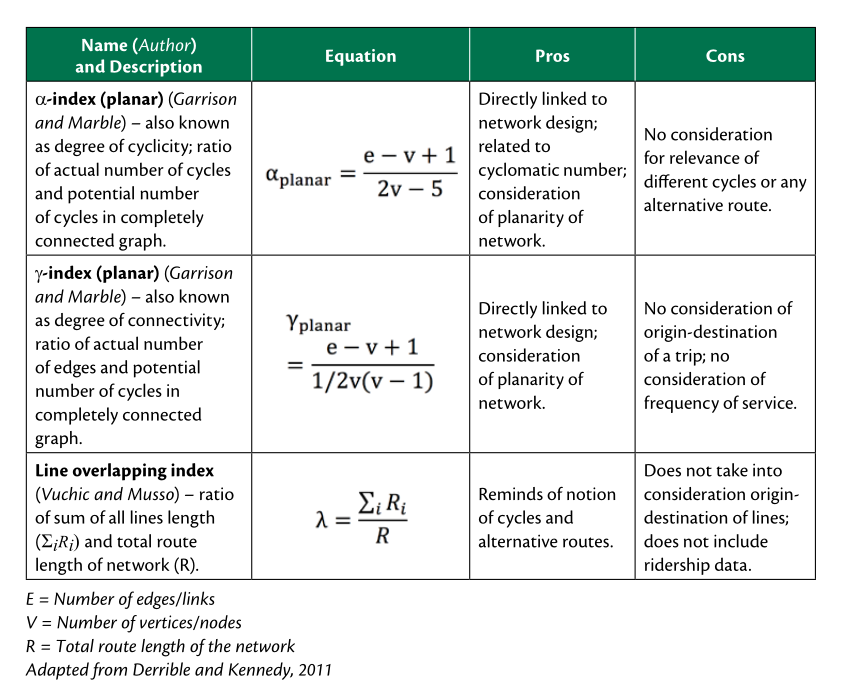
\includegraphics[width=0.85\textwidth]{Figures/Cap3/TablaIndicatorsAdaptedGraphTeory.png}
   \caption[Índices de Grafos \gtfs{}]{Tabla de indicadores de grafos \gtfs{}.
   Traducción: \textit{Name (Author) and Description}, nombre (autor) y
   descripción; \textit{Equation}, ecuación; \textit{Pros}, ventajas;
   \textit{Cons}, desventajas. Los índices son el $\alpha$ planar o grado de
   ciclicidad y el $\gamma$ planar o grado de conectividad, ambos de Garrison y
   Marble, y el índice de superposición de líneas, de Vuchic y Musso; $e$ es el
   número de aristas, $v$ el de vértices y $R$ la longitud total de las rutas.
   Tabla adaptada de Derrible y Kennedy (2011).}
   \label{fig:indices-grafos}
   \fuentefigura{\citet{fortin2016innovative}, p.~23.}
\end{figure}

Además de la eficiencia y la accesibilidad, la literatura mide la integración
entre modos. Se habla de interconectividad entre redes cuando metro, autobús,
trolebús, \brt{} y otros modos funcionan como un solo sistema, con transbordos
cortos y una cobertura que ninguno alcanzaría por su cuenta. En el grafo, esa
integración se dibuja con \termino{aristas de transferencia} entre nodos de
modos o líneas distintos; su peso incluye el tiempo de caminar entre andenes, la
espera y, si existe, una segunda tarifa.

\citet{ugur2025} afirman que la integración juega un papel crucial para
garantizar que los diferentes modos de transporte público operen de manera
armoniosa, facilitando las transferencias y permitiendo a los pasajeros
desplazarse con facilidad entre destinos. En un sistema bien integrado, la
fortaleza de la conexión entre líneas no solo amplía el área accesible para el
usuario, sino que también reduce las dificultades experimentadas durante el
viaje, lo que influye positivamente en la demanda de transporte público y
contribuye a la sustitución del vehículo privado. Su investigación sobre la
línea M7 del metro de Estambul demuestra que la evaluación sistemática de la
conectividad en cada estación ---mediante un
\termino{Índice de Conectividad Simplificado} (\textsc{sci}, por sus siglas en
inglés) que incorpora variables de velocidad, capacidad de pasajeros,
frecuencia, horas de operación y distancia al origen--- revela patrones de
integración desigual que orientan directamente las decisiones de inversión y
mejora operativa. La Figura~\ref{fig:sci-estambul} muestra el trazo de esa
línea y sus 17 estaciones.

\begin{figure}[H]
  \centering
  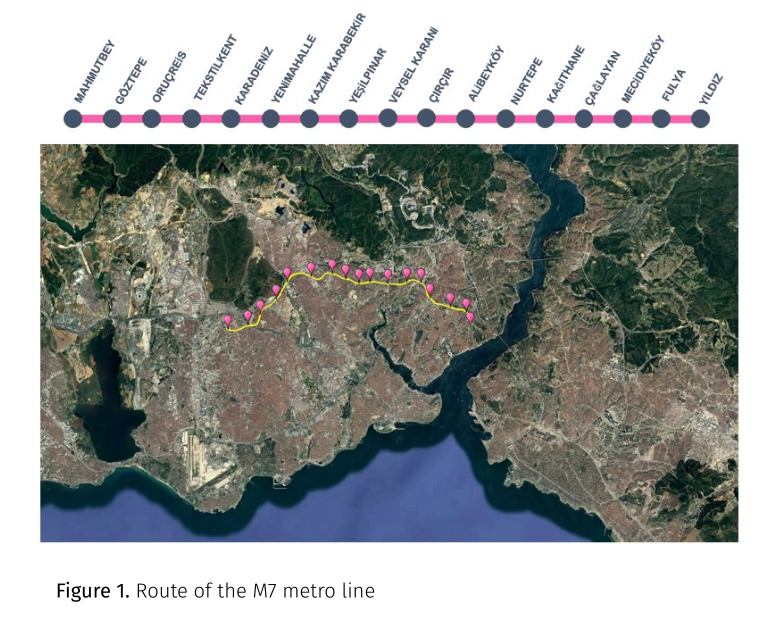
\includegraphics[width=0.88\textwidth]{Figures/Cap3/M7Estambul.png}
  \caption[Línea M7 del metro de Estambul]{%
  Trazo de la línea M7 del metro de Estambul y sus 17 estaciones, sobre la que
  \citet{ugur2025} calculan el \textsc{sci}. Traducción del rótulo:
  \textit{Route of the M7 metro line}, trazo de la línea M7 del metro;
  «Figure~1» es la numeración de la fuente.}
  \label{fig:sci-estambul}
  \fuentefigura{\citet{ugur2025}.}
\end{figure}

Para medir la interconectividad no basta contar cuántas líneas pasan por un
nodo; hay que medir qué tan buena es la conexión. \citet{mishra2015} evalúan la
conectividad en tres niveles: la parada, la línea y el centro de transferencia
(\termino{transfer center}). El índice de un nodo se obtiene de la suma de las
potencias de conexión de las líneas que pasan por él, y la potencia de cada
línea depende de su velocidad, distancia, frecuencia, tiempo de encabezamiento
(\termino{headway}), capacidad, aceleración y desaceleración, además de la
dirección de la ruta. Con esto, la eficiencia topológica y la operativa quedan
en una sola métrica por nodo, que esta tesis toma como referencia para construir
sus indicadores.

Este enfoque supera las limitaciones de la centralidad de grado simple, que
únicamente cuenta el número de conexiones directas de un nodo sin considerar la
calidad ni la frecuencia del servicio ofrecido. \citet{mishra2015} subrayan que
medir la conectividad puede resultar una tarea compleja y esquiva, pues es
necesario considerar tarifas, horarios, capacidad, frecuencia y otras
características del sistema en su conjunto; por ello, la evaluación de la
conectividad del transporte requiere un enfoque sistemático que integre los
múltiples parámetros involucrados en la prestación del servicio real. La
diferencia entre un sistema integrado y uno fragmentado se traduce directamente
en la magnitud de la \termino{penalización por transbordo} percibida por el
usuario: cuando la conectividad en los nodos de transferencia es alta, esta
penalización se reduce, haciendo el sistema más atractivo respecto al
automóvil.

Estos trabajos miden dimensiones distintas de la red: \citet{fortin2016innovative}
la eficiencia y la accesibilidad con los horarios reales del servicio,
\citet{batista2015} la concentración de los flujos en pocos nodos, y
\citet{mishra2015} y \citet{ugur2025} la calidad de la conexión en cada parada.
Cuando se quiere ver varias de esas dimensiones a la vez, la salida no es
obvia. \citet{kujala2018} normalizaron los datos \gtfs{} de 25 ciudades y
presentaron sus indicadores como un perfil por ciudad, sin reducirlos a un
índice global. Esa decisión es la que retoma la Clasificación Garibelt
(§\ref{subsubsec:garibelt-normalizacion}).

% !TeX root = ../../tesis.tex
% §2.1.4 — sustituye 2-3-Marco-Dispersion.tex l. 37-61 y 2-4-Teoria-Casos.tex
% l. 26-59 (#36). «Transiciones de Fase» (repetía 1-4) se eliminó; Aldous sale de §3.3.4.

% -----------------------------------------------------------------------
\subsection{Topología Anillo-Radial y Casos de Anillos}
\label{subsec:ea-anillo-radial}
% -----------------------------------------------------------------------

La teoría de redes ofrece dos argumentos para agregar un anillo a una red
radial. \citet{aldous2019optimal} buscan la geometría que minimiza el tiempo
promedio de viaje entre pares de puntos y encuentran que, cuando la longitud
total de la red rebasa un valor crítico $L_c$, la topología óptima cambia de
golpe y pasa a incluir un bucle o anillo. Su modelo es idealizado: indica cuándo
un anillo podría convenir, no dónde trazarlo. \citet{owais2020} llega a la misma
geometría por otra vía. Muestra que, en un sistema sobre todo radial, un anillo
reduce los transbordos necesarios para ir de una zona periférica a otra, con lo
que se acortan los traslados y el viaje multimodal pierde fricción.

\label{sec:casos-similares}
Dos metrópolis con redes radiales saturadas en el centro han optado por esa
geometría, con propósitos distintos. La Gran Línea Circular del Metro de Moscú,
inaugurada en 2023 con 70 kilómetros, se diseñó para descargar las líneas
radiales del centro y comunicar zonas periféricas sin pasar por las estaciones
centrales más congestionadas \citep{efe2023}. El \termino{Suburban Rail Loop} de
Melbourne, todavía en planeación y construcción, parte de otro diagnóstico: los
suburbios del \termino{Middle-Ring} concentran hospitales, universidades y
centros de empleo, pero no tienen conexiones laterales entre sí, y el proyecto
busca convertirlos en una red policéntrica de precintos de empleo
\citep{suburbanrailloop2021}. En Moscú el anillo resuelve un problema de
operación del centro; en Melbourne, uno de articulación de la periferia. Ninguna
de las dos fuentes mide la estructura de la red con indicadores como los de
§\ref{subsec:ea-indicadores}: una es una nota de prensa sobre la inauguración y
la otra resume el caso de negocio de un proyecto que aún no opera.

De estos casos se sabe que la geometría que esta tesis prueba sobre el Anillo
Periférico ya se eligió en otras metrópolis con problemas parecidos. No se sabe
cuánto cambia una red cuando se le agrega. Eso es lo que mide el
Capítulo~\ref{ch:analisis-red-anillo} para la \zmvm{}, con el anillo como caso
de demostración metodológica.

% !TeX root = ../../tesis.tex
% §2.1.5 — síntesis nueva (D36-4) + 2-5-SIG-Datos-Abiertos.tex l. 82-102 (D36-6) (#36)

% -----------------------------------------------------------------------
\subsection{Síntesis: Tendencias, Debates y Vacíos}
\label{subsec:ea-sintesis}
% -----------------------------------------------------------------------

La tendencia más clara es tratar la red de transporte como un grafo construido
con datos \gtfs{}. \citet{fortin2016innovative} cargan los \termino{feeds} en
una base de grafos para calcular caminos mínimos e indicadores;
\citet{kujala2018} normalizan con el mismo estándar las redes de 25 ciudades, y
\citet{ugur2025} miden la conectividad estación por estación. La segunda
tendencia es el \termino{software} propio y abierto. \citet{moreno2023}
defienden el desarrollo modular en Python para que una institución acumule
capacidad de análisis sin pagar licencias, y la cartografía colaborativa ya
cubre buena parte de la red vial de las ciudades latinoamericanas grandes
\citep{barrington2017world}.

Hay dos debates abiertos. El primero es cómo resumir varias dimensiones de una
red. Un índice compuesto da una sola cifra, pero un valor alto en una dimensión
puede tapar uno bajo en otra \citep{hossain2024}, y en redes multimodales la
concentración de flujos en pocos nodos se pierde dentro del índice
\citep{deng2023}. Por eso \citet{kujala2018} prefirieron un perfil por ciudad,
y esta tesis toma el mismo partido con la Clasificación Garibelt
(§\ref{subsubsec:garibelt-compensabilidad}). El segundo debate enfrenta la
demanda con la estructura. El Programa Maestro del Metro de 1985 midió con
detalle la demanda; con ella, los corredores del Periférico no alcanzaban la
captación que se exigía, y la evaluación no podía registrar lo que un anillo
aporta a la estructura de la red (§\ref{subsubsec:anillo-pm-2010}). Esta tesis
mide la estructura y deja fuera la demanda, de modo que ninguno de los dos
enfoques basta solo.

Quedan tres vacíos. El primero: de los anillos de otras metrópolis se conoce el
propósito, pero no hay una medición de la red (§\ref{subsec:ea-anillo-radial}).
El segundo está en los datos. \citet{haklay2010good} y
\citet{barrington2017world} miden la completitud de la red vial, no la de las
paradas de transporte, y en la \zmvm{} los sistemas que operan solo en el
Estado de México no tienen \gtfs{} oficial (§\ref{subsec:limitaciones-datos}).
El tercero es de herramientas. En México el \termino{software} propio de
análisis apenas empieza; el del Instituto Mexicano del Transporte se presenta
como primera etapa y trata la asignación de tráfico \citep{moreno2023}. Es la
brecha que describe \citet{gurstein2011open}: los datos abiertos sirven poco si
no hay herramientas para quien no programa.

\label{subsec:datos-herramienta-replicable}
Esta investigación responde a esa brecha con una cadena de tres motores de
código abierto. \texttt{Apímetro} reúne y normaliza los \termino{feeds}
\gtfs{}, \texttt{VFTModel} calcula los indicadores y
\texttt{Transport-gis-zmvm-mjg} los lleva a mapas que un urbanista puede leer sin
saber programar. Ninguno depende de licencias comerciales, y la cadena se puede
repetir en cualquier área metropolitana con \termino{feeds} \gtfs{} y
cartografía \gis{} de base, algo que, según \citet{barrington2017world}, cumple
la mayoría de las ciudades latinoamericanas de escala comparable a la \zmvm{}.

El argumento de replicabilidad no es secundario, sino central al objetivo
general de la investigación: demostrar que un planificador urbano con acceso a
datos abiertos puede, mediante esta metodología, obtener un diagnóstico
topológico riguroso de su red de transporte y evaluar escenarios alternativos de
intervención sin depender de \termino{software} propietario ni de equipos técnicos
especializados. Los referentes de calidad de datos
\citep{haklay2010good, barrington2017world} y los principios de equidad en el
acceso al conocimiento \citep{gurstein2011open, neis2012street} constituyen, en
este sentido, el fundamento teórico que articula la dimensión metodológica de la
tesis con su dimensión urbanística.


% !TeX root = ../../tesis.tex
%%%%%%%%%%%%%%%%%%%%%%%%%%%%%%%%%%%%%%%%%%%%%%%%%%%%%%%%%%%%%%%%%%%
% §2.2 ANTECEDENTES HISTÓRICOS — ARCHIVO PADRE — EN BLANCO
% Estructura prevista (descomentar al llenar):
% \section{Antecedentes Históricos}
% \label{sec:antecedentes-historicos}
% % !TeX root = ../../tesis.tex
%%%%%%%%%%%%%%%%%%%%%%%%%%%%%%%%%%%%%%%%%%%%%%%%%%%%%%%%%%%%%%%%%%%
% §2.2.1 LA HEGEMONÍA DEL AUTOMÓVIL — EN BLANCO
% Origen: 2-MarcoTeorico/2-1-Apertura-Hegemonia.tex (59 l.):
%   - l. 5-39  apertura histórica (tranvías, Revolución, urbanismo); hoy
%     va antes de la primera \section. Pasa a ser el primer bloque aquí.
%   - l. 41-59 «La Hegemonía del Automóvil y la adopción de la
%     automovilidad» (\label{sec:hegemonia-automovil}: se conserva,
%     ahora como subsección).
%   Autores: molina2018, biblioteca1935, franco2022, perlo2023.
% El \chapter y \label{ch:marco-teorico} de l. 3-4 pasan al padre
%   2-MarcoTeorico.tex con el título «Estado del Arte y Marco Teórico».
%%%%%%%%%%%%%%%%%%%%%%%%%%%%%%%%%%%%%%%%%%%%%%%%%%%%%%%%%%%%%%%%%%%

% % !TeX root = ../../tesis.tex
%%%%%%%%%%%%%%%%%%%%%%%%%%%%%%%%%%%%%%%%%%%%%%%%%%%%%%%%%%%%%%%%%%%
% §2.2.2 EL ANILLO PERIFÉRICO: UN PROYECTO POLÍTICO ESTRUCTURAL — EN BLANCO
% Origen: 2-MarcoTeorico/2-2-Anillo-Periferico.tex (110 l., completo):
%   - l. 4-19   entrada (\label{sec:anillo-periferico})
%   - l. 20-59  «Centralización Administrativa y… XII Cuarteles»
%   - l. 60-81  «La Prioridad Presupuestal: El Sesgo Vial Hegemónico»
%               (subsec:sesgo-vial, citado en 7.2)
%   - l. 82-110 «El Déficit Estructural y el Rechazo al Metro»
%               (subsec:rechazo-metro, citado en 7.2)
%   Autores: franco2022, perlo2023.
% Al mover: bajar un nivel los títulos y conservar todos los \label.
%%%%%%%%%%%%%%%%%%%%%%%%%%%%%%%%%%%%%%%%%%%%%%%%%%%%%%%%%%%%%%%%%%%

%%%%%%%%%%%%%%%%%%%%%%%%%%%%%%%%%%%%%%%%%%%%%%%%%%%%%%%%%%%%%%%%%%%

% !TeX root = ../../tesis.tex
%%%%%%%%%%%%%%%%%%%%%%%%%%%%%%%%%%%%%%%%%%%%%%%%%%%%%%%%%%%%%%%%%%%
% §2.3 MARCO TEÓRICO — ARCHIVO PADRE — EN BLANCO
% Estructura prevista (descomentar al llenar):
% \section{Marco Teórico: Dispersión, Fragmentación y Equidad}
% \label{sec:marco-teorico}
% % !TeX root = ../../tesis.tex
%%%%%%%%%%%%%%%%%%%%%%%%%%%%%%%%%%%%%%%%%%%%%%%%%%%%%%%%%%%%%%%%%%%
% §2.3.1 DISPERSIÓN, FRAGMENTACIÓN Y MODELO RADIAL — EN BLANCO
% Origen: 2-MarcoTeorico/2-3-Marco-Dispersion.tex (61 l.):
%   - l. 4-22  entrada de la sección (padilla2007, molinero2002)
%   - l. 23-36 «Limitaciones del Modelo Radial»
%   (l. 37-61 pasan a 2-1-4-Anillo-Radial; l. 40-44 se eliminan por
%   repetir 1-4 l. 124-128.)
% Revisar al mover: \label de la sección y quién la cita.
%%%%%%%%%%%%%%%%%%%%%%%%%%%%%%%%%%%%%%%%%%%%%%%%%%%%%%%%%%%%%%%%%%%

% % !TeX root = ../../tesis.tex
% §2.3.2 — movido de 2-MarcoTeorico/2-4-Teoria-Casos.tex l. 3-24 (#36)

\phantomsection\label{sec:teoria-latinoamericana}

Para enmarcar el caso de la \cdmx{} en un contexto de crítica urbanística
regional, es fundamental recurrir a la teoría sobre la ciudad en América Latina.
La obra compilatoria de \citet{padilla2007} proporciona el marco conceptual para
entender que la crisis de movilidad en la periferia es síntoma de un agotamiento
del modelo de planeación estatal y la adopción de enfoques que favorecieron el
capital inmobiliario y la privatización del espacio. La incapacidad de la
planeación urbana para gestionar la expansión territorial generada por los
grandes proyectos viales, como el Periférico, es el caldo de cultivo para la
emergencia de la ciudad neoliberal.

El escenario de un corredor anillar constituye, en este contexto teórico, un
caso de demostración metodológica: permite evaluar si la transición de un
enfoque radial ---propio de la era Uruchurtu--- hacia uno que incorpora
geometrías transversales reduce cuantitativamente los indicadores de
ineficiencia topológica que aquejaban a la ciudad fragmentada
\citep{franco2022}.

%%%%%%%%%%%%%%%%%%%%%%%%%%%%%%%%%%%%%%%%%%%%%%%%%%%%%%%%%%%%%%%%%%%

